\documentclass[11pt,a4paper]{article}

\usepackage[margin=2.4cm]{geometry}
\usepackage{amsmath,amssymb,mathtools}
\usepackage{booktabs}
\usepackage{graphicx}
\usepackage{xcolor}
\usepackage{hyperref}
\usepackage{enumitem}
\usepackage{array}
\usepackage{algorithm}
\usepackage{algpseudocode}

\hypersetup{
  colorlinks=true,
  linkcolor=blue!55!black,
  urlcolor=blue!55!black
}

\newcommand{\R}{\mathbb{R}}
% Notation revised 2026-09-19 (supervisor review): the original \F and \M
% collide with standard robotics usage (F = force, M = the mass/inertia
% matrix M(q) in the rigid-body equations of motion), and the neighbourhood
% set had been sharing \N with the Gaussian N(mu,Sigma) used throughout the
% MPPI sections -- an internal clash, not just an external one. Fixed by:
% \F  (free cells)      -> \Free, rendered Omega (a free/feasible region,
%                          standard in optimization/motion-planning texts;
%                          avoids C, already used in Algorithm 1 for the
%                          raw costmap input).
% \M  (outward boundary) -> written directly as the topological boundary
%                          operator applied to \B_rho, i.e. \partial\B_\rho,
%                          rather than a new letter -- it IS the boundary of
%                          the flood body, so this is not a notational
%                          choice, it's the same object under its standard
%                          name. No new macro needed.
% \N  (neighbours)       -> kept exclusively for the Gaussian; the 8-cell
%                          neighbourhood now uses \Adj_8(p) (graph-theoretic
%                          "adjacency"), typographically distinct (upright,
%                          not calligraphic) from the Gaussian \N(.,.).
\newcommand{\Free}{\Omega}
\newcommand{\B}{\mathcal{B}}
\newcommand{\N}{\mathcal{N}}
\newcommand{\Adj}{\operatorname{Adj}}
\newcommand{\Path}{\mathcal{P}}
\newcommand{\dist}{\operatorname{dist}}
\newcommand{\clip}{\operatorname{clip}}

\title{Mathematics of Topology-Guided MPPI\\
\large A Geodesic Flood-Field Construction for Multimodal Biased MPPI}
\author{Topology-Guided MPPI sandbox notes}
\date{\today}

\begin{document}
\maketitle

\begin{abstract}
This document develops the mathematical construction used to turn a local
occupancy map into a geodesically reachable flood region, its outward
boundary, and a small set of topology-distinct branch centrelines. It
deliberately separates physical reachability from navigation preference. The
final section shows how a branch becomes an ancillary control proposal for
Biased MPPI. The equations describe the present discrete sandbox
implementation; they are not a proof of full kinodynamic reachability.
(For continuity with the accompanying codebase and demonstration videos,
which predate this terminology, the implementation is internally named
\texttt{amoeba\_sandbox}; this document uses geometry-first terminology
throughout.) Notation follows standard motion-planning/MPC usage rather than
overloading letters already reserved elsewhere in robotics (e.g.\ force,
a rigid body's mass matrix); see Section~\ref{sec:notation}.
\end{abstract}

\tableofcontents
\newpage

\section{What the construction computes}

Let $x_r=(p_r,\theta_r)$ be the robot state, with planar position
$p_r=[x_r,y_r]^\top$. The construction pipeline computes
\begin{equation}
\text{obstacle map}
\longrightarrow \Free
\longrightarrow \B_\rho(p_r)
\longrightarrow \partial\B_\rho
\longrightarrow \{P_1,\ldots,P_M\}.
\end{equation}
Here $\Free$ is collision-free position space, $\B_\rho$ is a local geodesic
ball, $\partial\B_\rho$ is its outward flood boundary, and $P_m$ is one topological-branch
centreline. The stages answer different questions:
\begin{description}[leftmargin=3.1cm,style=nextline]
  \item[Body] Which nearby positions are connected to the robot through free
  space within a finite travel budget?
  \item[Flood boundary] Where does that travel budget expire while free space
  continues?
  \item[Navigation field] Which flood-boundary exits appear useful for
  reaching the global objective?
  \item[Topological branches] Which useful exits correspond to genuinely
  different local routes?
\end{description}

\section{Discrete local grid}

The continuous plane is sampled on a square grid with resolution
\begin{equation}
  \Delta r = 0.05\ \mathrm{m}.
\end{equation}
This is the distance between adjacent cell centres, not the flood-body radius.
The grid coordinate $(i,j)$ represents
\begin{equation}
  p_{ij}=
  \begin{bmatrix}
  x_0+i\Delta r\\ y_0+j\Delta r
  \end{bmatrix}.
\end{equation}
If the geodesic reach is $\rho=2.5\,\mathrm{m}$, then a straight unobstructed
radius spans approximately
\begin{equation}
  \frac{\rho}{\Delta r}=\frac{2.5}{0.05}=50
\end{equation}
grid transitions.

\subsection{Collision-free cells}

Let $c(p)$ be the Euclidean distance from position $p$ to the nearest
obstacle. For a circular planning footprint of radius $r_p$, define
\begin{equation}
  \Free=\{p_{ij}:c(p_{ij})>r_p\}.
  \label{eq:free}
\end{equation}
Equation~\eqref{eq:free} is a configuration-space approximation: obstacles
are effectively inflated by $r_p$, after which the robot is treated as a
point. In the provisional rectangular V6 model, the orientation-free global
and geodesic layers use
\begin{equation}
  r_p=\frac{W}{2}+m_{\mathrm{turn}}
      =\frac{0.65}{2}+0.08=0.405\ \mathrm{m}.
\end{equation}
The full oriented rectangle is checked later during control rollout. The
circular proxy does not prove that every orientation is feasible.

\section{Eight-connected grid graph}

Treat every free cell as a graph vertex. A cell may connect to its horizontal,
vertical, and diagonal free neighbours. For an offset
$(\delta_i,\delta_j)\in\{-1,0,1\}^2\setminus\{(0,0)\}$, the edge length is
\begin{equation}
  w(\delta_i,\delta_j)
  =\Delta r\sqrt{\delta_i^2+\delta_j^2}.
\end{equation}
Consequently,
\begin{align}
  w_{\mathrm{straight}}&=\Delta r=0.05\ \mathrm{m},\\
  w_{\mathrm{diagonal}}&=\sqrt{2}\Delta r\approx0.0707\ \mathrm{m}.
\end{align}
Different edge lengths are why ordinary breadth-first search is insufficient:
it would treat a diagonal step as equal to a straight step.

\section{Robot-centred geodesic distance}

For any free cell $p$, define the discrete geodesic distance
\begin{equation}
  d_r(p)=
  \min_{\gamma:p_r\leadsto p}
  \sum_{e\in\gamma}w(e),
  \label{eq:reach-distance}
\end{equation}
where every vertex of path $\gamma$ must lie in $\Free$. Dijkstra's algorithm
computes Equation~\eqref{eq:reach-distance} from the robot to all locally
reachable cells:
\begin{align}
  d_r(p_r)&=0,\\
  d_r(p)&=\infty \quad \text{initially for }p\ne p_r,\\
  d_r(q)&\leftarrow
  \min\bigl(d_r(q),d_r(p)+w(p,q)\bigr).
\end{align}

\subsection{Why Dijkstra rather than A*?}

A* efficiently seeks one specified target using
\begin{equation}
  f(p)=g(p)+h(p).
\end{equation}
The construction does not yet know its useful endpoints. It needs the
distance to \emph{every} reachable local cell, so a single-source,
all-destinations Dijkstra expansion is the natural operation. One result
supports body construction, flood-boundary detection, endpoint ranking, and
branch backtracing. A* remains appropriate for the separate global
start-to-goal plan.

\section{The geodesic body}

The body is the sublevel set of robot-centred geodesic distance:
\begin{equation}
  \boxed{
  \B_\rho(p_r)=\{p\in\Free:d_r(p)\leq\rho\}.
  }
  \label{eq:body}
\end{equation}
In open space $d_r(p)$ approximately equals Euclidean distance, so the body
appears nearly circular. Near obstacles,
\begin{equation}
  d_r(p)\geq\lVert p-p_r\rVert_2,
\end{equation}
with strict inequality when a route must detour. Therefore the body bulges
into open space, stops at obstacles, pinches through narrow passages, and
wraps around obstacles. The parameter $\rho$ is a local foresight budget:
increasing it reveals more topology but costs more computation and may expose
more irrelevant branches.

\paragraph{Important limitation.}
Equation~\eqref{eq:body} represents connected, collision-free
\emph{position} reachability. It does not include heading, velocity,
acceleration, non-holonomic constraints, or skid-steer slip. Those are tested
later when a branch is converted into a control sequence.

\section{How the flood region moves with the robot}

The flood region is not a rigid shape translated with the robot. At rebuild cycle
$k$, the current robot position becomes a new geodesic source and the complete
construction is repeated:
\begin{equation}
  p_r^{(k)}
  \longrightarrow d_r^{(k)}(p)
  \longrightarrow \B_\rho^{(k)}
  \longrightarrow \partial\B_\rho^{(k)}
  \longrightarrow \{P_m^{(k)}\}.
  \label{eq:moving-rebuild}
\end{equation}
Consequently, nearby obstacles continually reshape the body and can create,
merge, or remove topological branches. In the sandbox the field is normally rebuilt
every five controller cycles. With $\Delta t=0.05\,\mathrm{s}$, that is a
nominal rebuild interval of
\begin{equation}
  5\Delta t=0.25\,\mathrm{s}.
\end{equation}
The MPPI loop uses the most recently built field between rebuilds.

Figure~\ref{fig:amoeba-motion} is generated from a successful execution of the
actual sandbox controller in BARN world 48. The pale-blue region is
$\B_\rho$, cyan points show $\partial\B_\rho$, blue arrows show descent of the navigation
value, dotted coloured curves are extracted branch centrelines, the black
disc is the robot, and red is the already driven trajectory.

\begin{figure}[ht]
  \centering
  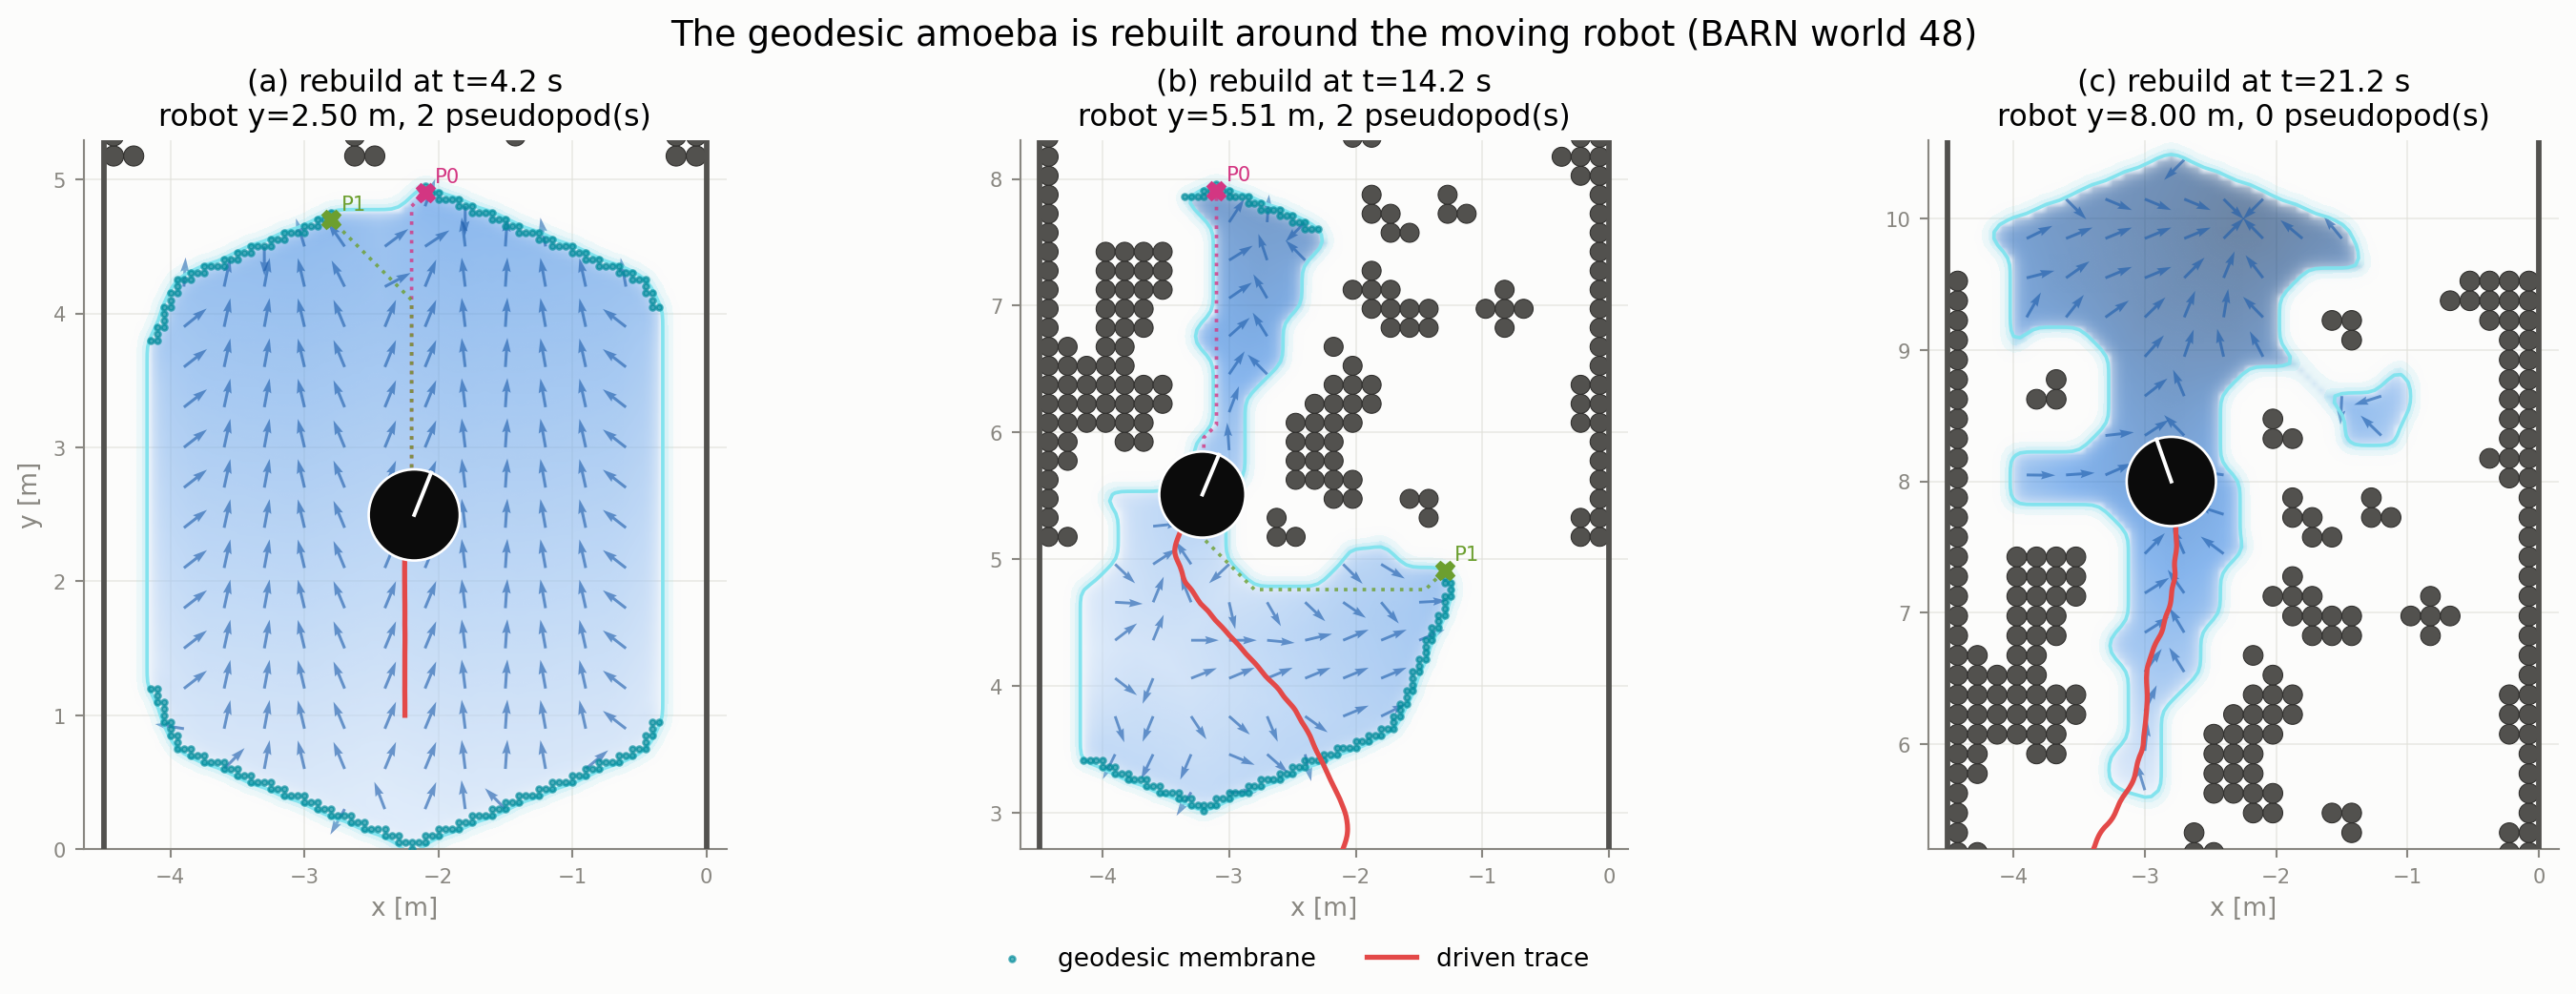
\includegraphics[width=\textwidth]{../artifacts/images/demos/amoeba_motion_sequence.png}
  \caption{Three implementation-derived snapshots of the rolling geodesic
  flood region. In open space (a), the body is broad. In clutter (b),
  obstacles deform and split its reachable extensions, producing alternative
  topological branches. Near the goal (c), the goal lies inside the local
  body, so the navigation field is seeded directly at the goal and no
  outward flood-boundary branches are required. The apparent smooth cyan
  outline is a plotting interpolation; all planning calculations use the
  underlying $0.05\,\mathrm{m}$ grid.}
  \label{fig:amoeba-motion}
\end{figure}

This sequence also clarifies what ``applied to the geodesic flood region''
means. The plain reach-distance expansion decides the blue support region.
The flood-boundary costs seed the second, narrow-channel-weighted flood
inside that support. Its downhill directions rank and guide local
continuation, while the distinct flood-boundary backtraces provide the
geometries later converted into ancillary control sequences.

\section{The outward flood boundary}

Let $\Adj_8(p)$ denote the eight grid neighbours of $p$. The outward
flood boundary is
\begin{equation}
  \boxed{
  \partial\B_\rho=
  \left\{
  p\in\B_\rho:
  \exists q\in\Adj_8(p),\quad
  q\in\Free\setminus\B_\rho
  \right\}.
  }
  \label{eq:membrane}
\end{equation}
Thus a flood-boundary cell borders free space that the geodesic budget did
not reach. A body cell adjacent only to an obstacle is not automatically a
useful outward flood-boundary cell. This distinction prevents wall
boundaries from being mistaken for possible local exits.

\section{Flood-boundary cost: the ``promise'' value}

When the goal lies outside the local body, the navigation flood cannot be
seeded directly at the goal. Each $m\in\partial\B_\rho$ is instead assigned a terminal
cost-to-go estimate $h(m)$. ``Promise'' is only an intuitive name: it is a
heuristic cost, not a guarantee, probability, or reward. Lower is better.

\subsection{Goal-distance boundary cost}

Without a global path,
\begin{equation}
  h(m)=\lVert m-p_g\rVert_2.
  \label{eq:goal-promise}
\end{equation}
This prefers flood-boundary locations geometrically closer to the goal, but cannot
see obstacles beyond the local body.

\subsection{Global-path boundary cost}

Let the global path be $\Path=\{z_0,\ldots,z_N\}$, and let
$L_{\mathrm{rem}}(z_k)$ be its remaining arclength from $z_k$ to the goal.
Then
\begin{equation}
  h(m)=
  \min_{z_k\in\Path}
  \left[
  \lVert m-z_k\rVert_2+L_{\mathrm{rem}}(z_k)
  \right].
  \label{eq:path-promise}
\end{equation}
The first term estimates reconnection cost; the second estimates the
subsequent route to the goal. The global path ranks flood-boundary exits but
does not replace the true local free-space domain.

\section{Obstacle narrow-channel weight and the navigation field}

Physical reach and navigation preference are deliberately different. Define
an obstacle-dependent narrow-channel weight
\begin{equation}
  \eta(p)=1+\alpha\,
  \clip\left(
  1-\frac{c(p)-r_p}{b},0,1
  \right),
  \label{eq:viscosity}
\end{equation}
where $\alpha\geq0$ is the weight strength and $b>0$ is the clearance band.
Near inflated obstacles $\eta$ is large; in open space it approaches one.
A weighted edge may be written
\begin{equation}
  w_\eta(p,q)=w(p,q)\eta(q).
\end{equation}
The navigation value inside the body is the multi-source shortest-path field
\begin{equation}
  \boxed{
  D_g(p)=
  \min_{m\in\partial\B_\rho}
  \left[
  h(m)+d_\eta(p,m)
  \right].
  }
  \label{eq:navigation-field}
\end{equation}
Equivalently, every flood-boundary cell is inserted into Dijkstra's priority queue
with initial value $h(m)$, and weighted distances propagate inward.
The negative gradient $-\nabla D_g$ supplies a goal-seeking local direction.

The separation is essential:
\begin{align}
  d_r(p)&:\ \text{plain geodesic distance used for physical reach},\\
  D_g(p)&:\ \text{narrow-channel-weighted value used for route preference}.
\end{align}
Using the narrow-channel weight in $d_r$ would shrink the physical body
precisely in narrow, high-resistance passages where forward visibility is
important.

\section{Branch endpoint selection}

Every valid flood-boundary cell is a potential endpoint. The implementation ranks
candidates using
\begin{equation}
  s(m)=D_g(m)+d_r(m).
  \label{eq:branch-score}
\end{equation}
On the seeded flood boundary $D_g(m)=h(m)$, so this balances estimated continuation
and travel from the robot. Candidates within a score slack of the best value
are considered. Spatial non-maximum suppression then requires
\begin{equation}
  \lVert m_i-m_j\rVert_2\geq d_{\mathrm{end}}
\end{equation}
for retained endpoint candidates, avoiding many nearly identical endpoints
on the same flood-boundary arc.

\section{Centreline tracing and topology filtering}
\label{sec:centreline-topology}

For each endpoint $m_i$, a centreline is traced toward the robot by repeatedly
moving to a neighbouring cell with lower $d_r$:
\begin{equation}
  p_{k+1}\in
  \arg\min_{q\in\Adj_8(p_k)}d_r(q).
  \label{eq:backtrace}
\end{equation}
After reversing the trace,
\begin{equation}
  P_i=[p_r,p_{i,1},\ldots,m_i].
\end{equation}

Endpoint separation alone does not establish distinct topology: two endpoints
may lie far apart in the same open room. The sandbox resamples two candidate
centrelines, finds locations where their separation exceeds a threshold, and
tests connectors between corresponding points. If a connector crosses dry
space, the routes are treated as separated by an obstacle and therefore
topologically distinct. This is a practical local test, not a formal homotopy
proof.

The output is at most $M$ topological branches,
\begin{equation}
  \{P_1,\ldots,P_M\},\qquad M\leq3,
\end{equation}
with IDs tracked between field rebuilds.

\section{From branch to ancillary controller}

The geometry $P_m$ is converted by a branch-following policy $\mathcal A$ into
a complete control-sequence mean:
\begin{equation}
  \mu_m=\mathcal A(P_m,x_0)
  =[u_{m,0},\ldots,u_{m,T-1}],
  \qquad u_{m,t}=[v_{m,t},\omega_{m,t}]^\top.
  \label{eq:ancillary-mean}
\end{equation}
A schematic tracking law is
\begin{align}
  e_{\theta,m,t}
  &=\operatorname{wrap}
  (\theta^{\mathrm{target}}_{m,t}-\theta_{m,t}),\\
  \omega_{m,t}
  &=k_\theta e_{\theta,m,t}+k_\kappa\kappa_{m,t},\\
  v_{m,t}
  &=v_{\max}
  g_h(e_{\theta,m,t})g_\kappa(\kappa_{m,t})g_c(c_{m,t}).
\end{align}
Velocity and acceleration limits are enforced, and the sequence is rolled
through the same motion and footprint model used by MPPI. An infeasible
sequence is not promoted to an active proposal mode.

\section{Connection to Biased MPPI}

Each feasible ancillary sequence becomes the mean of a proposal component:
\begin{equation}
  q_m(U)=\N(U;\mu_m,\Sigma_m).
\end{equation}
Together with a protected global-path or nominal fallback, the sampling
distribution is
\begin{equation}
  q(U)=\sum_{m=0}^{M}\pi_m q_m(U).
  \label{eq:mixture}
\end{equation}
For the path-integral target
\begin{equation}
  p^*(U)\propto
  \exp\left(-\frac{S(U)}{\lambda}\right)p(U),
\end{equation}
the full importance-corrected log weight is
\begin{equation}
  \log\widetilde w_k
  =-\frac{S(U_k)}{\lambda}
   +\log p(U_k)-\log q(U_k).
  \label{eq:importance}
\end{equation}
The topology-guided contribution is therefore upstream of MPPI weighting: it converts
local free-space topology into the ancillary means $\mu_m$ in
Equation~\eqref{eq:mixture}. Mode-conditioned updates preserve left/right
route alternatives instead of averaging controls across an obstacle.

\subsection{Frozen NumPy thesis estimator}

Equation~\eqref{eq:importance} is the formally corrected V4 alternative, but
it is \emph{not} the estimator used for the frozen thesis results. The V4/V4.1
ablations exposed severe finite-sample ESS collapse, so the final benchmark
uses fixed covariance and the stable V3 grouped, mode-conditioned estimator.
Let $\mathcal A_k$ be the feasible branch modes exposed by the NORMAL/ASSIST
gate at control cycle $k$, and let mode $0$ be the protected A*-path fallback:
\begin{equation}
  \mathcal Q_k=\{0\}\cup\mathcal A_k,
  \qquad q_m(U)=\N(U;\mu_m,\Sigma).
\end{equation}
If $M_k=|\mathcal A_k|>0$, the frozen NumPy allocation is
\begin{equation}
  \pi_0=0.25,
  \qquad
  \pi_m=\frac{0.75}{M_k},\quad m\in\mathcal A_k;
  \qquad N_m\simeq\pi_mN.
  \label{eq:frozen-allocation}
\end{equation}
If no branch is exposed, $\pi_0=1$ and the complete batch samples the path
fallback. Within each fixed group, the uncorrected MPPI weights and free energy
are
\begin{align}
  w_{i\mid m}
  &=\frac{\exp[-(S(U_i)-S_{m,\min})/\lambda]}
          {\sum_{j:z_j=m}\exp[-(S(U_j)-S_{m,\min})/\lambda]},\\
  F_m
  &=-\lambda\log\!\left[
       \frac{1}{N_m}\sum_{i:z_i=m}\exp(-S(U_i)/\lambda)
     \right].
  \label{eq:frozen-mode-evidence}
\end{align}
The committed-mode state machine selects $m^*$ from the mode free energies,
subject to minimum dwell, improvement margin, and multi-cycle confirmation.
The control mean is updated \emph{only inside the selected topology}:
\begin{equation}
  U^*=\sum_{i:z_i=m^*}w_{i\mid m^*}U_i,
  \qquad u_k=(U^*)_0.
  \label{eq:frozen-selected-update}
\end{equation}
Thus good left and right routes are never averaged into a control through the
obstacle between them.

The final comparators follow directly. Path-cost MPPI (\texttt{path\_mppi})
changes $S(U)$ but keeps ordinary nominal sampling -- it is \emph{not} Biased
MPPI, despite the similar name, since sampling itself is untouched.
Single-path Biased MPPI (\texttt{path\_biased}) is the true literature
comparator: it uses only $q_0(U)=\N(U;\mu_{\mathrm{A*}},\Sigma)$ and samples
the whole batch around the A*-derived ancillary mean. Full TG-MPPI uses that identical protected fallback
in NORMAL, and augments it with the topology-distinct $q_m$ components in
ASSIST. Flow-only retains geodesic cost/bias but sets $\mathcal A_k=\varnothing$.

\section{Parallel global-route topology extension}

Everything above describes topology inside one rolling geodesic body. A
separate, PyTorch-only exploratory pilot (\texttt{torch\_port}, not the
sandbox or Nav2 port that produced any validated result in this document)
extends the same idea one level up: several whole-route global A* topologies
$\mathcal R=\{R_0,\ldots,R_{K-1}\}$ (rejecting near-duplicates by
nearest-point separation) run as separate MPPI groups, each with its own
free energy $F_z$ under the same committed-mode selection rule as
Equation~\eqref{eq:frozen-mode-evidence}, plus a long-horizon route-conflict
prior for two cooperating robots comparing announced routes beyond the
$2.8\,$s local rollout horizon. This is real, implemented, geometric-diversity
work, but it is a separate research thread, not part of the single-robot
static or dynamic-obstacle results elsewhere in this document, and is not
detailed further here.

\subsection{Current Nav2 Phase~3 realization}

The C++ port implements the same geometric idea with a guarded partial-batch
bias. Let $N$ be the Nav2 MPPI batch size and $\alpha$ the maximum ancillary
fraction. The ancillary budget and vanilla budget are
\begin{equation}
  N_a=\lfloor\alpha N\rfloor,\qquad N_0=N-N_a.
\end{equation}
Currently $N=2000$ and $\alpha=0.20$, giving at most 400 ancillary samples and
approximately 1600 ordinary MPPI samples. For active branch promise values
$h_m$, the allocation probabilities are
\begin{equation}
  \pi_m=\frac{\exp(-h_m/\tau_p)}
              {\sum_j\exp(-h_j/\tau_p)},
  \qquad \tau_p=0.75,
\end{equation}
and mode $m$ receives approximately $N_a\pi_m$ samples. Lower terminal cost
therefore receives more samples, but no promise is interpreted as a guarantee.
Each assigned row is recentered around the full time-varying sequence
$\mu_m=[u_{m,0},\ldots,u_{m,T-1}]$; it is not merely given one constant steering
offset. The unassigned rows retain the vanilla Nav2 proposal, providing a
large fallback population.

This is the implemented proposal mechanism, not yet a complete independent
mode-selection system. Nav2's existing critics still score the resulting
rollouts, and the separate flow critic is disabled in the current test
configuration. The next safety requirement is explicit footprint/costmap
validation of each ancillary mean and its realized rollout before treating it
as a valid proposal component.

\section{Space-time topology extension}
\label{sec:spacetime}

Every construction above floods free \emph{space}: a topological branch or
global route is a curve through $\R^2$, and two curves are treated as distinct when
an obstacle separates them at every shared point. A moving obstacle is not
representable this way. It only enters through the MPPI cost as a
time-indexed clearance term -- the sandbox's own \texttt{mppi.py} V6.1
prediction layer (documented in the companion progress notes,
\texttt{docs/amoeba\_mppi\_progress.tex}) and, in the live Nav2 port, the
\texttt{DynamicObstacleCritic} formalized in
Section~\ref{sec:dynamic-obstacle-cost} below -- so ``wait for it to pass''
and ``go before it arrives'' are never offered as candidate means $\mu_m$ by
that cost term alone; they must be discovered by sampling noise around
whichever single branch mean already exists, or supplied explicitly as extra
modes by the space-time search this section formalizes. This section
formalizes flooding free \emph{space-time} instead, so a predicted
obstacle's swept path becomes a tube that separates routes the same way a
pillar does. This is the implemented mechanism (\texttt{spacetime.py} in the
sandbox, \texttt{tools/space\_time\_search.cpp} in the Nav2 port), not yet
integrated with the geodesic body $\B_\rho$ above or the global-route
extension $\mathcal R$: it operates on one topological branch or path
reference at a time.

\subsection{Predicted-obstacle collision cost (Nav2 port)}
\label{sec:dynamic-obstacle-cost}

This is the per-rollout-point term that actually keeps the controller clear
of moving obstacles; the space-time construction that follows only
\emph{proposes} extra candidate means, it does not itself avoid anything
(Section~\ref{sec:spacetime-empirical} makes this distinction precise, with
measurements). It
is a direct MPPI-cost restatement of the dynamic-obstacle constraint in de
Groot, Ferranti, Gavrila and Alonso-Mora, ``Topology-Driven Parallel
Trajectory Optimization in Dynamic Environments'' (T-MPC), \emph{RA-L}
(their Eq.~2d/14): a hard per-timestep constraint there becomes a soft
per-rollout-point cost here, so it composes with MPPI's Monte-Carlo cost
accumulation instead of a gradient-based constrained optimizer. \textbf{This
term's formulation is not original to this project}; the contribution, such
as it is, is the restatement and the Nav2/xtensor implementation
(\texttt{tools/dynamic\_obstacle\_cost.hpp},
\texttt{critics/DynamicObstacleCritic}).

For rollout $i$, point $j=1,\ldots,T$ reached after $j$ controls, let
$t_j=\min(j\,\Delta t,\,T_{\max})$ be that point's time-since-now under the
model's own step $\Delta t$ (a clamp, not a physical cutoff: the constant-
velocity estimate is simply not trusted past $T_{\max}$). The footprint is
represented as two discs, offset $\pm\delta$ along the rollout's heading
$\psi_j$ from the robot centre, each of radius $r_f$ (fit to the
$0.84\times0.68\,$m rectangle: $\delta=0.21\,$m, $r_f=\sqrt{0.21^2+0.34^2}
\approx0.40\,$m). For tracked obstacle $k$ with position $o_k$, velocity
$v_k$ (constant-velocity extrapolation, Equation~\eqref{eq:spacetime-free}'s
$\hat o(\tau)$ specialized to this critic's own $t_j$), and radius $r_k$,
the signed clearance of disc offset $\epsilon\in\{+\delta,-\delta\}$ is
\begin{equation}
  d_{j,k,\epsilon}=
  \bigl\lVert\, p_j+\epsilon\,[\cos\psi_j,\sin\psi_j]-(o_k+v_k t_j)\,\bigr\rVert_2
  -(r_f+r_k),
  \label{eq:dynobs-clearance}
\end{equation}
and $d_j=\min_{k,\epsilon}d_{j,k,\epsilon}$ the worst clearance at that point
over every tracked obstacle and both discs. Per-point cost is
\begin{equation}
  c(d_j)=
  \begin{cases}
    c_{\mathrm{coll}}+c_{\mathrm{pen}}\,\lvert d_j\rvert, & d_j<0,\\[4pt]
    c_{\mathrm{crit}}\left(\dfrac{d_{\mathrm{soft}}-d_j}{d_{\mathrm{soft}}}\right)^{2}, & 0\le d_j<d_{\mathrm{soft}},\\[6pt]
    0, & d_j\ge d_{\mathrm{soft}},
  \end{cases}
  \label{eq:dynobs-cost}
\end{equation}
a quadratic repulsive band inside $d_{\mathrm{soft}}$ and a large fixed
penetration cost \emph{plus} a term proportional to overlap depth once
already colliding -- graded, not flagged infeasible and discarded, so among
several already-bad rollouts MPPI's softmax still prefers the least
penetrating one (the ``least-bad escape'' the header comment names it) --
and the rollout's total dynamic-obstacle cost is
\begin{equation}
  J_{\mathrm{dyn}}(i)=w_{\mathrm{dyn}}\left(\frac{1}{T}\sum_{j=1}^{T}c(d_j)\right)^{p},
  \label{eq:dynobs-total}
\end{equation}
added into the same cost sum every other critic contributes to before the
softmax weighting of Equation~\eqref{eq:frozen-selected-update} (or its
un-mixed single-mode equivalent when grouped sampling is off). Defaults:
$d_{\mathrm{soft}}=0.5\,$m (speed-scaled to the braking distance
$v_{\max}^2/2a$ at higher $v_{\max}$), $c_{\mathrm{crit}}=300$,
$c_{\mathrm{coll}}=10^6$, $c_{\mathrm{pen}}=10^4$, $w_{\mathrm{dyn}}=3.81$,
$p=1$.

\subsection{Time-expanded state space}

Let $\Delta t_\ell$ be the time-layer spacing and $\Delta r_s$ the search's
own spatial resolution, generally coarser than the flood's $\Delta r$. A
state is a triple $(p,k)$, position $p\in\R^2$ at discrete time
$\tau_k=k\Delta t_\ell$, $k=0,\ldots,K$, $K=\lfloor T_s/\Delta t_\ell\rfloor$
for search horizon $T_s$. Transitions advance exactly one layer: an ordinary
move $(p,k)\to(q,k+1)$ for $q\in\Adj_8(p)$, or a \emph{wait}
$(p,k)\to(p,k+1)$. Because every transition advances $k$ by one regardless of
whether $p$ changes, waiting costs real time exactly as moving does -- this
is what lets ``wait'' be a genuine competing strategy rather than a free
action.

Let $\hat o(\tau)\in\R^2$ be one predicted obstacle's position at time $\tau$
(e.g.\ \texttt{dynabarn.py}'s constant-velocity extrapolation from its last
observed position and velocity) and $r_o$ its radius. A state is free when
\begin{equation}
  c(p)>r_p
  \quad\text{and}\quad
  \lVert p-\hat o(\tau_k)\rVert_2>r_p+r_o,
  \label{eq:spacetime-free}
\end{equation}
the same static test as Equation~\eqref{eq:free} together with
a synchronized-time exclusion disc around the predicted obstacle. A path
$\pi=[(p_0,0),\ldots,(p_K,K)]$ is feasible when every state satisfies
Equation~\eqref{eq:spacetime-free} and, for diagonal moves, both flanking
orthogonal cells are free at the arriving layer (the same no-corner-cutting
rule as the global A* planner).

\subsection{Cost and the wait/detour construction}

For a step $(p,k)\to(q,k+1)$, the cost is
\begin{equation}
  c(p,q)=
  \begin{cases}
    \Delta r_s\lVert q-p\rVert_2/\Delta r_s, & q\ne p,\\[2pt]
    c_w, & q=p,
  \end{cases}
  \label{eq:spacetime-step-cost}
\end{equation}
and a path's cost is $\sum_k c(p_k,p_{k+1})$. The cheapest feasible path is
found by Dijkstra over $(p,k)$ exactly as in Equation~\eqref{eq:reach-distance},
now with the extra time coordinate.

Bounding \emph{which} layer counts as arrival (an early deadline
$k\le k_{\max}$ vs.\ a late one $k\ge k_{\min}$) was tried and rejected: it
degenerates whenever reaching the goal safely is possible well before
$k_{\min}$, since the cheapest way to satisfy a late deadline is then simply
to arrive early and idle, physically the same route wrongly labelled
distinct. A deadline changes which path \emph{qualifies}, not which one is
cheapest. Varying the wait cost $c_w$ changes which path \emph{is} cheapest,
so it does not degenerate this way. Solving Equation~\eqref{eq:spacetime-step-cost} twice,
once with $c_w=c_w^{\text{cheap}}$ (waiting favoured) and once with
$c_w=c_w^{\text{expensive}}$ (moving favoured, so a lateral detour becomes
the cheaper way to avoid the same obstacle), gives
\begin{equation}
  \pi_{\mathrm{wait}}=\Pi(c_w^{\text{cheap}}),\qquad
  \pi_{\mathrm{detour}}=\Pi(c_w^{\text{expensive}}),
  \label{eq:two-route}
\end{equation}
where $\Pi(c_w)$ denotes the Dijkstra solution under that wait cost. Verified
on a synthetic crossing (one obstacle traversing the corridor once): the
cheap-wait solution held position for several layers with a $0.2\,$m lateral
excursion, while the expensive-wait solution never waited and swung $0.6\,$m
to the side -- two genuinely different strategies, not a relabelling of one.

\subsection{Synchronized-time distinctness}

Section~\ref{sec:centreline-topology}'s distinctness test asks whether a
connector between two static centrelines crosses dry space -- it compares
positions with no notion of time. A moving obstacle only separates two
routes that pass its location at genuinely \emph{different} times, so the
comparison must synchronize on $\tau$. For paths $\pi_a,\pi_b$ (padded by
holding the shorter one at its final position, the physical situation of
having already arrived), define at each shared layer $k$
\begin{equation}
  d_a=p_{a,k}-\hat o(\tau_k),\qquad
  d_b=p_{b,k}-\hat o(\tau_k).
  \label{eq:spacetime-side-vectors}
\end{equation}
The routes are distinct when some layer with both $\lVert d_a\rVert_2$ and
$\lVert d_b\rVert_2$ within a relevance radius $r_{\mathrm{rel}}$ satisfies
\begin{equation}
  d_a\cdot d_b<0,
  \label{eq:spacetime-distinct}
\end{equation}
i.e.\ the obstacle sits between them at a moment when it is actually close to
both -- the temporal analogue of Section~\ref{sec:centreline-topology}'s dry-
space-crossing test, evaluated at synchronized time instead of position (this
implementation's cost-based mode-purity term against a static obstacle uses
the same side-of-obstacle principle, evaluated at closest approach instead of
per step; see \texttt{homotopy.py}). This flag is diagnostic only: a
symmetric scenario can let both routes drift to the same side of the
obstacle (Equation~\eqref{eq:spacetime-distinct} false) while still being
procedurally different (one holds position, the other does not), so
$\{\pi_{\mathrm{wait}},\pi_{\mathrm{detour}}\}$ are offered as candidate
modes on feasibility alone, never gated on Equation~\eqref{eq:spacetime-distinct}.

\subsection{Empirical distinctness rate and root cause}
\label{sec:spacetime-empirical}

The diagnostic caveat above understates the problem. Live Nav2 measurement
(15 dynamic-scenario trials, $\approx$11{,}000 crossing detections) found
Equation~\eqref{eq:spacetime-distinct} true in only a few dozen cases: about
96\% of detections were flagged non-distinct, and a standalone synthetic
harness (head-on crossings at three lateral offsets and three obstacle
speeds, both searches genuinely feasible in 9/9) found the equation true in
only 2/9. Widening $r_{\mathrm{rel}}$ recovered almost none of the rest
(5/9 stayed non-distinct even at $1.6\,$m).

This is not sampling noise; it is what
Equation~\eqref{eq:spacetime-distinct} actually asks. A pass-before route and
a pass-behind route are close to the obstacle at \emph{different} layers $k$
by construction -- one crosses the obstacle's line of motion before it
arrives, the other after it has gone -- so at any single shared layer
\emph{usually only one} route satisfies $\lVert d_a\rVert_2\le r_{\mathrm{rel}}$
or $\lVert d_b\rVert_2\le r_{\mathrm{rel}}$, and
Equation~\eqref{eq:spacetime-distinct} is vacuously unevaluated at every
other layer. The test is structurally blind to exactly the distinction it
exists to detect: it asks whether two routes are on opposite sides of the
obstacle \emph{at the same time}, when the thing that actually separates a
wait route from a detour route is which side of the obstacle's line of
motion each route occupies at \emph{its own} crossing moment -- a
\emph{crossing-order} invariant, the space-time analogue of a winding
number, not a synchronized-side test. A corrected test would label each
route independently at its own closest-approach layer $k^\star_a$
(respectively $k^\star_b$) by the sign of
$\bigl(p_{a,k^\star_a}-\hat o(\tau_{k^\star_a})\bigr)\cdot v_o$ (projection
onto the obstacle's own velocity: positive means the obstacle has not yet
reached that point, negative means it already has) and declare the routes
distinct when the two signs differ -- not attempted here, filed as the
concrete fix candidate.

A second, independent cause compounds the first even when a distinct pair
\emph{is} found: the grouped-sampling selection of Equation~\eqref{eq:mixture}
is winner-takes-all across groups, and a proposal group's expected free-energy
minimum scales as $-\sigma\sqrt{2\ln N}$ in its own sample count $N$. At the
Nav2 port's default allocation (fallback $N\approx1600$ against
$N\approx80$--$130$ per active mode) the unbiased fallback wins by roughly
$0.9\sigma$ of sample-count advantage alone -- above the $0.3\sigma$ switch
margin -- so even a genuinely distinct, genuinely better proposal can lose
the softmax purely to being outnumbered, independent of whether it is
correct. Giving every active group (including the fallback) a near-equal
share of the batch, which is the sandbox's own default allocation rule and
an opt-in parameter in the port (\texttt{tgmppi\_group\_allocation:equal}),
removes this term, but was not observed to change the live outcome
materially on its own -- consistent with the first cause dominating.

\subsection{Trigger and local goal}

Recomputing Equation~\eqref{eq:two-route} every cycle for every branch is
unnecessary: it is only worth it when the existing reference $\mu_m$ would
actually collide with a predicted obstacle. Extending $\mu_m$'s branch
centreline at the search's own implied speed $v_s=\Delta r_s/\Delta t_\ell$
gives a check trajectory $\{p(\tau_k)\}_{k=0}^{K}$ along the centreline arc
length; the branch triggers a space-time alternative when
\begin{equation}
  \min_{k,\,j}\bigl[
    \lVert p(\tau_k)-\hat o_j(\tau_k)\rVert_2-(r_p+r_{o,j})
  \bigr]\le0
  \label{eq:spacetime-trigger}
\end{equation}
for any tracked obstacle $j$ -- the worst (most negative) margin selects
which single obstacle the search is built against, matching
Equation~\eqref{eq:spacetime-free}'s single-obstacle exclusion test. The search
target is not the branch's full, possibly distant endpoint -- which
Equation~\eqref{eq:two-route} treats as a hard arrival requirement, unlike the
receding-horizon partial-progress tracking $\mathcal A$ performs in
Equation~\eqref{eq:ancillary-mean} -- but a point reachable at $90\%$ of $v_s$
within the search horizon $T_s$, arc-length interpolated along the same
centreline. Two evaluation windows -- the check trajectory here fixed at
$v_s$, the search grid also implied speed $v_s$ -- must agree, or a goal
picked as ``reachable'' or a crossing checked over the wrong horizon each
silently return \emph{infeasible} or \emph{no trigger} for a reason that has
nothing to do with the obstacle -- both were real bugs found before the
mechanism ever produced a route, and are why the two windows are stated
here as a matching requirement rather than left implicit.

\subsection{Extending the proposal set}

A feasible route from Equation~\eqref{eq:two-route} is resampled onto the
controller's own grid $(T,\Delta t)$ by linear interpolation (holding the
final position beyond the route's own duration), differenced into
$[v,\omega]$ commands, and projected through the same box/rate limits as
$\mathcal A$ in Equation~\eqref{eq:ancillary-mean} -- producing a mean
$\mu_{m,\mathrm{wait}}$ or $\mu_{m,\mathrm{detour}}$ with exactly the same
type as any other branch mean. Holding a wait segment through this
resampling matters: collapsing repeated identical points as a zero-length
segment (as $\mathcal A$ does for an ordinary polyline) would discard the one
piece of information a wait route exists to carry. For a triggered branch
$m$, the active label set of Equation~\eqref{eq:mixture} extends to
\begin{equation}
  \mathcal Z_t\leftarrow\mathcal Z_t\cup
  \{m_{\mathrm{wait}},m_{\mathrm{detour}}\}\setminus
  \{z:z\text{ infeasible}\},
  \label{eq:spacetime-mode-extension}
\end{equation}
each with the same conditional weights and free energy as any other label
(Equations~\eqref{eq:frozen-mode-evidence}--\eqref{eq:frozen-selected-update}),
subject to the same minimum-dwell, improvement-margin, and multi-cycle
confirmation hysteresis, with no special-casing.

\subsection{Scope}

Implemented for one topological branch against one predicted obstacle at a
time: several simultaneous obstacles collapse to the single worst one in
Equation~\eqref{eq:spacetime-trigger}, and the path fallback does not yet
receive a space-time alternative.

\textbf{Now validated against a scripted dynamic-obstacle benchmark}
(\texttt{thesis\_dyn}: 5 open-room worlds $\times$ 3 conditions $\times$ 3
reps at 0.3--1.0\,m/s obstacles; \texttt{thesis\_dyn\_fast}: 2 worlds at
human-walking-pace 1.2--1.4\,m/s obstacles). The honest result: full TG-MPPI
(with the space-time and pseudopod mechanisms of this section and
Section~\ref{sec:centreline-topology} both active) is statistically
indistinguishable from Section~\ref{sec:dynamic-obstacle-cost}'s
predicted-obstacle collision cost run alone, on legs completed, contact
rate, clearance, and speed (Spearman/Fisher tests, $p=0.08$--$1.0$ across
metrics at $n=15$--$21$ per condition), while either configuration beats
stock Nav2 MPPI overwhelmingly ($p<10^{-7}$). Consistent with
Section~\ref{sec:spacetime-empirical}: space-time selections occurred in
only 12--17 of $\approx$11{,}000 detections across the run. The gain over
stock in dynamic scenes is attributable to
Equation~\eqref{eq:dynobs-total} alone, not to this section's guidance
mechanism, in open-room scenes of this kind. This mirrors the static-BARN
finding of Section~\ref{sec:centreline-topology} exactly: branch selection
measured $0.000$ across the ten-world static generality matrix there too --
the pseudopod/space-time guidance layer is validated as \emph{correct and
inert} in both settings tested to date, not yet as improving anything, and
its demonstrated value (the blocked-path McNemar result, $9/10$ vs $2/10$,
$p=0.0156$) lives specifically in the locally-blocked-path regime, which
neither of these Gazebo benchmarks reproduces.

\section{Topology-guided biased MPPI algorithm}

Algorithm~\ref{alg:amoeba-mppi} gives the compact, paper-style construction
corresponding to the guarded partial-batch Nav2 realization. The first part is
evaluated at the flood-field update rate; the final sampling, rollout, and
weighting steps occur in each MPPI control cycle. The frozen NumPy estimator is
given separately by Equations~\eqref{eq:frozen-allocation}--
\eqref{eq:frozen-selected-update}; it selects and updates one mode rather than
combining all modes in one Nav2 update.

\begin{algorithm}[ht]
\caption{Geodesic Topology-Guided Ancillary Proposals for Biased MPPI}
\label{alg:amoeba-mppi}
\begin{algorithmic}[1]
\Require Costmap $C$, robot state $x_r=(p_r,\theta_r)$, goal $p_g$,
global path $\Path$, reach $\rho$, footprint proxy $r_p$, batch size $N$,
horizon $T$, ancillary fraction $\alpha_a$, promise temperature $\tau_p$
\Ensure Applied control $u_0^*$
\State $\Free \gets \{p\in C:c(p)>r_p\}$
\State $d_r \gets \Call{Dijkstra}{p_r,\Free,w}$
\State $\B_\rho \gets \{p\in\Free:d_r(p)\leq\rho\}$
\State $\partial\B_\rho \gets \{p\in\B_\rho:\Adj_8(p)\cap(\Free\setminus\B_\rho)\neq\varnothing\}$
\ForAll{$m\in\partial\B_\rho$}
  \State $h(m)\gets\displaystyle\min_{z_k\in\Path}
  \bigl(\lVert m-z_k\rVert_2+L_{\mathrm{rem}}(z_k)\bigr)$
\EndFor
\State $\eta(p)\gets 1+\alpha_\eta\,
\clip\!\left(1-\dfrac{c(p)-r_p}{b},0,1\right)$, $\forall p\in\B_\rho$
\State $D_g(p)\gets\displaystyle\min_{m\in\partial\B_\rho}
\left[h(m)+d_\eta(p,m)\right]$, $\forall p\in\B_\rho$
\State $\mathcal E\gets\Call{NMS}{\operatorname{sort}_{m\in\partial\B_\rho}
\left(D_g(m)+d_r(m)\right)}$
\State $\{P_m\}_{m=1}^{M}\gets
\Call{DistinctBacktraces}{\mathcal E,d_r,\Free}$, $M\leq3$
\For{$m=1,\ldots,M$}
  \State $\mu_m\gets\Call{ProjectConstraints}{\mathcal A(P_m,x_r,T)}$
  \State $X_m\gets\Call{Rollout}{x_r,\mu_m}$
  \If{$X_m$ violates the footprint/costmap constraint}
    \State discard mode $m$ \Comment{required safety gate}
  \EndIf
\EndFor
\State $N_a\gets\lfloor\alpha_aN\rfloor,\qquad N_0\gets N-N_a$
\State $\pi_m\gets\dfrac{\exp(-h_m/\tau_p)}
{\sum_{j=1}^{M}\exp(-h_j/\tau_p)},\qquad
N_m\gets\Call{IntegerAllocate}{N_a\pi_m}$
\State $U^{(k)}\sim\N(\bar U,\Sigma_0)$,
$k=1,\ldots,N_0$ \Comment{vanilla fallback}
\For{$m=1,\ldots,M$}
  \State $U^{(k)}\sim\N(\mu_m,\Sigma_m)$ for the $N_m$ samples of mode $m$
\EndFor
\State $X^{(k)}\gets\Call{Rollout}{x_r,U^{(k)}},\qquad
S_k\gets\Call{Nav2Critics}{X^{(k)},U^{(k)}}$
\State $w_k\gets\dfrac{\exp[-(S_k-S_{\min})/\lambda]}
{\sum_j\exp[-(S_j-S_{\min})/\lambda]}$
\State $U^*\gets\Call{MPPIUpdate}{\{U^{(k)},w_k\}_{k=1}^{N}}$
\State \Return $u_0^*$
\end{algorithmic}
\end{algorithm}

If the goal lies inside $\B_\rho$, the navigation value is seeded directly
at the goal and the flood-boundary branch proposal stage may be omitted. If no
valid branch remains, set $N_a=0$ and recover ordinary Nav2 MPPI. The
footprint-rejection line is included as the mathematically required gate; its
complete integration into the current Nav2 port remains pending.

\section{Notation summary}
\label{sec:notation}

\begin{table}[h]
\centering
\begin{tabular}{>{\bfseries}p{0.18\linewidth}p{0.70\linewidth}}
\toprule
Symbol & Meaning \\
\midrule
$\Delta r$ & Grid resolution; currently $0.05\,\mathrm{m}$. \\
$r_p$ & Circular planning-footprint proxy. \\
$\rho$ & Geodesic flood reach; commonly $2.5\,\mathrm{m}$. \\
$c(p)$ & Clearance from position $p$ to the nearest obstacle. \\
$\Free$ & Collision-free grid cells. \\
$d_r(p)$ & Plain geodesic distance from the robot. \\
$\B_\rho$ & Flood body, the $\rho$-sublevel set of $d_r$. \\
$\Adj_8(p)$ & The 8-connected grid neighbours of $p$ (graph adjacency; kept
typographically distinct from the Gaussian $\N(\cdot,\cdot)$ below). \\
$\partial\B_\rho$ & Outward flood boundary where the geodesic budget expires
-- the topological boundary of $\B_\rho$, not a separate symbol. \\
$h(m)$ & Flood-boundary terminal cost-to-go estimate (``promise''). \\
$\eta(p)$ & Obstacle-dependent narrow-channel weight. \\
$D_g(p)$ & Narrow-channel-weighted navigation value inside the body. \\
$P_m$ & Topology-distinct branch centreline. \\
$\mu_m$ & Ancillary control-sequence mean generated from $P_m$. \\
$q_m(U)$ & MPPI proposal distribution conditioned on branch $m$. \\
$R_k$ & Global route topology candidate $k$. \\
$F_z$ & Conditional free energy of topology/proposal label $z$. \\
$J_k^{\mathrm{route\mbox{-}conflict}}$ & Long-horizon cooperative conflict prior for route $k$. \\
\bottomrule
\end{tabular}
\end{table}

\section{Key conceptual distinctions}

\begin{enumerate}[leftmargin=*]
  \item Grid resolution $\Delta r$ controls numerical detail; geodesic reach
  $\rho$ controls the physical extent of the local body.
  \item Collision-free grid construction is shared costmap preprocessing; it
  is not itself DWA, A*, or this method's novelty.
  \item Dijkstra is used because all local distances are needed. A* is used
  separately when one start-to-goal path is needed.
  \item The body uses plain distance to represent reach. The narrow-channel
  weight affects preference, not body membership.
  \item A promise value is a terminal cost estimate, never a guarantee.
  \item A flood-boundary endpoint is not automatically a distinct route.
  Geometry and dry-space separation are used to suppress equivalent branches.
  \item Geometric reachability is checked first; control and footprint
  feasibility are checked when generating the ancillary sequence.
\end{enumerate}

\end{document}
